\subsubsection{Login}
\subsubsection{Registration}
\subsubsection{Location Search}
The search service, is used to search and load any place in the world. As shown in the figure below, you need to click in the search box and start typing the name of the place you are searching for. \\[0.5cm]
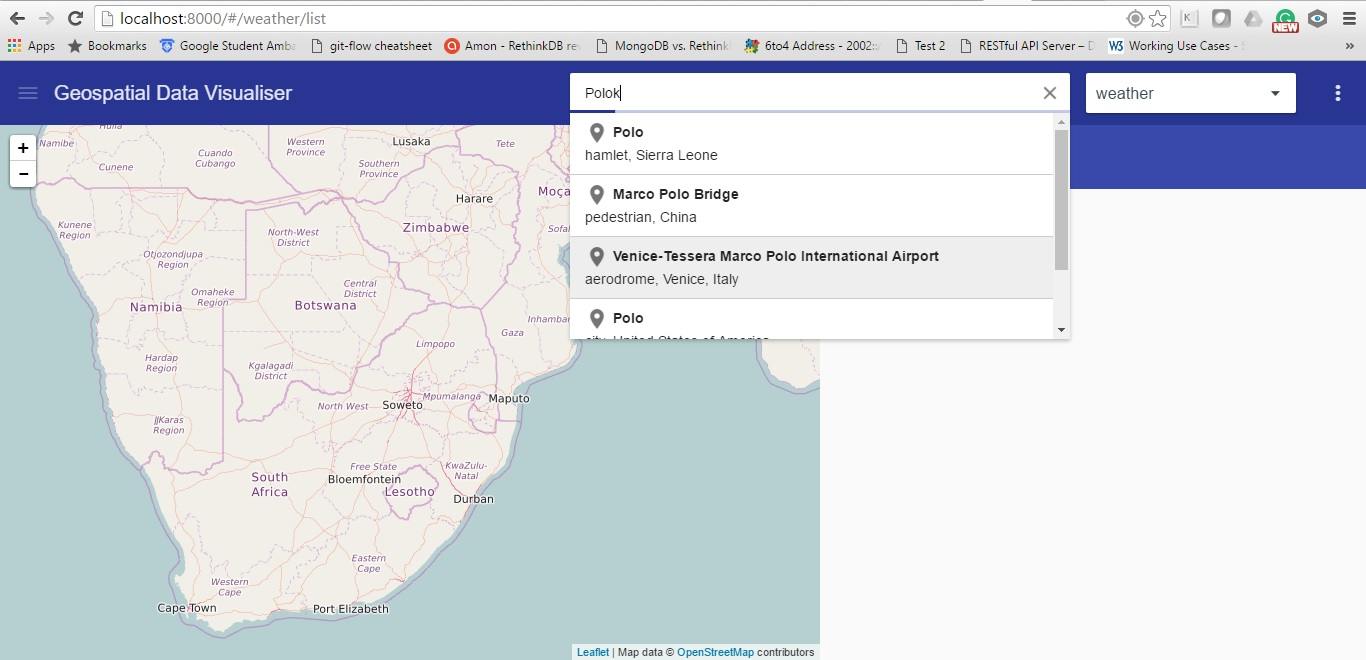
\includegraphics[width=\textwidth]{searchFunction} \\[0.5cm]
While searching a possible list of places will be loaded in a dropdown list as shown in the figure above. Once you have found the place you are looking for, use your mouse to point to the name of the place and click on that name, which will then activate a process of reloading the map to the place you have selected, like the figure shown below. A marker will be placed to show the location you queried. \\[0.5cm]
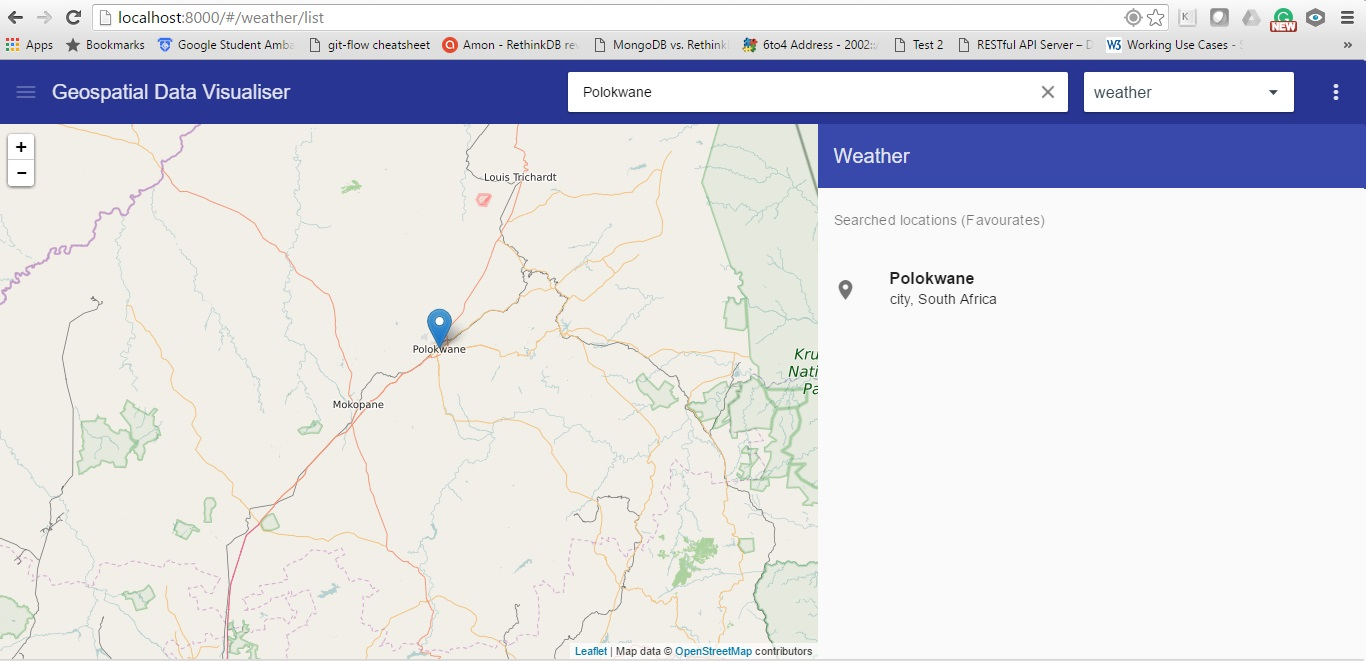
\includegraphics[width=\textwidth]{searchResult} \\[0.5cm]
The search feature is also linked to other functions of the site. When the weather center is currently active, the location name will be added to the listed of locations you have already searched for as shown above. These features will be explained in more detail in sections about the respective features.
\subsubsection{Disaster Center}
To navigate to the disaster center. Click on the "Center navigation" and move you mouse cursor over the "disasters" button on the dropdown list and click. Shown in the the figure below. \\[0.5cm]
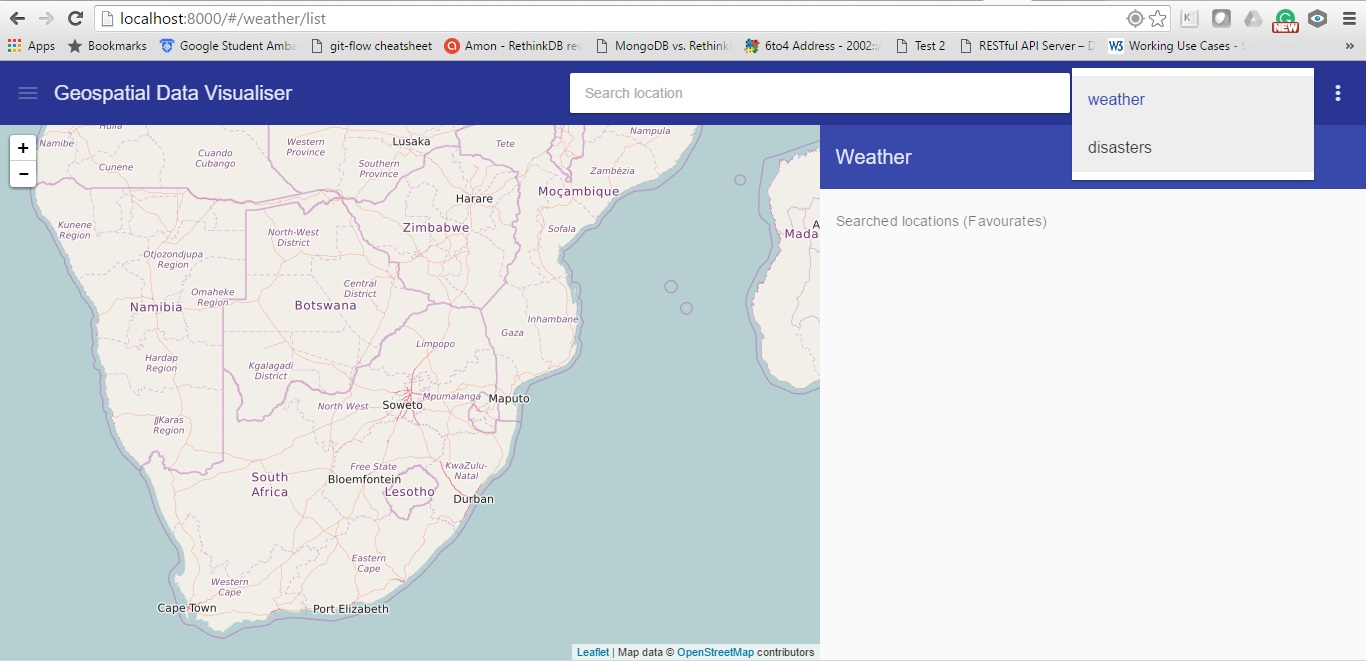
\includegraphics[width=\textwidth]{disaster1} \\[0.5cm]
Once you have loaded the disaster center, you will land on the page shown in the figure below below. The numbers on the figure show the features currently available in the disaster center. \\[0.5cm]
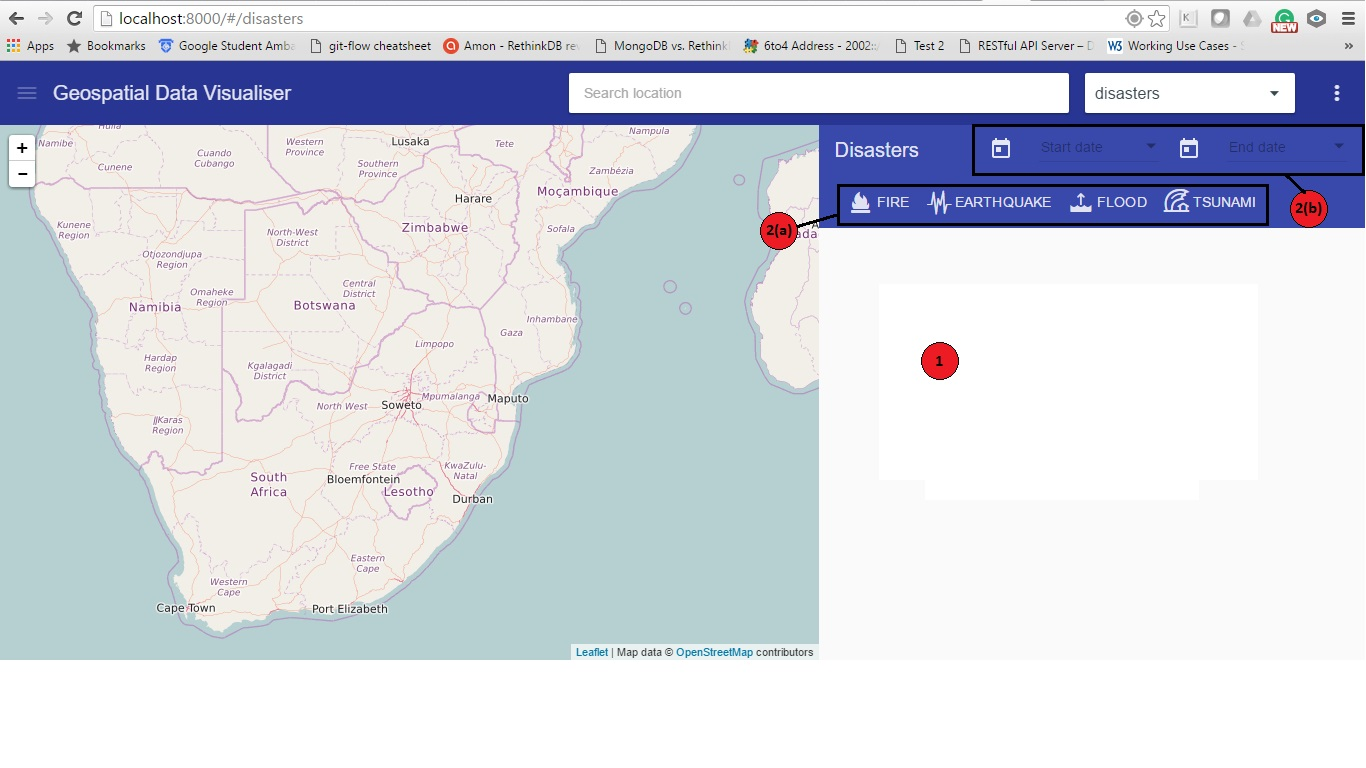
\includegraphics[width=\textwidth]{disaster2} \\[0.5cm]
	\begin{enumerate}
		\item \textbf{List of disasters} : This part of the center will show the list of disasters that are currently displayed on the map area. It will allow the user to load more information about each disaster displayed on the map area. For example, if a user decides to show earthquakes as shown in the figure below. The earthquakes or any disaster for that matter will be loaded on to the map area. The blue icons show a number of disasters clustered in a specific range of area the blue icon lays over. Each individual disaster then has its own type of icon. Earthquakes shown by yellow icons, fires by red etc. As you may see from the figure below, only the individual disasters are shown on the list. \\[0.5cm]
		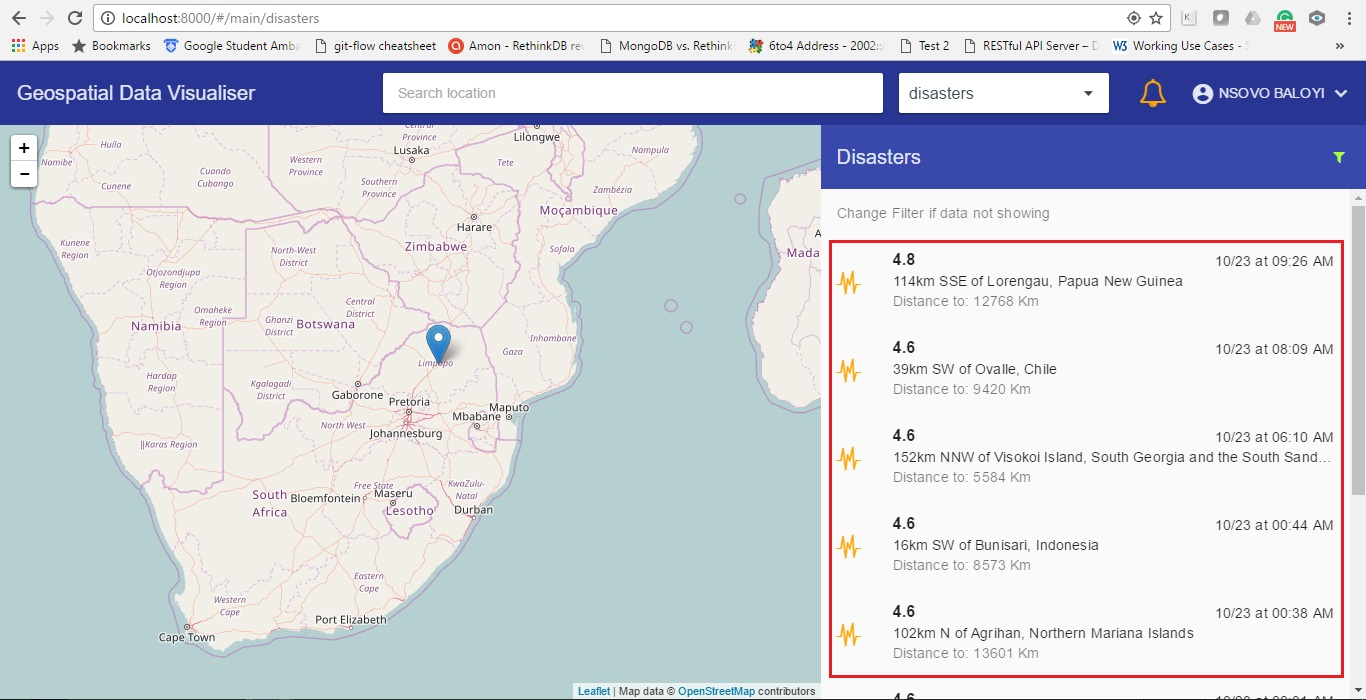
\includegraphics[width=\textwidth]{disaster3} \\[0.5cm]
		By moving the map to another location you then refresh the list by loading the disaster currently visible on the map area.
		\item \textbf{Query Features}
		This section describes how the query features may be used.
		\begin{enumerate}
		\item \textbf{Query by Type}: This feature allows you to query disasters by type. You may click on one or more of the buttons on the query panel, which will then perform a query and load the selected disasters on the map area. When clicked the system then performs a query for the type queried and displays it on the map. This will then reload the button in the "clicked" state. By clicking it again you the perform another query to remove the disaster you clicked on from the map area.
		\item \textbf{Query by Time}: This feature, like the the type query, will perform a query to load disasters which happen on the specified date. This allows the user to load disasters from a specified date in the past to the current date of the day the query is perform. This feature goes hand in hand with the type query, therefore if no disaster is picked, no disaster will be loaded  on the map area even after picking a date.
		\end{enumerate}
		As stated above, once a query is performed, the disasters are loaded onto the map area. The blue icons show the number of disasters clustered in a range that is projected by the blue section that appears when you hover over one of the blue icons as shown in the figure below. \\[0.2cm]
		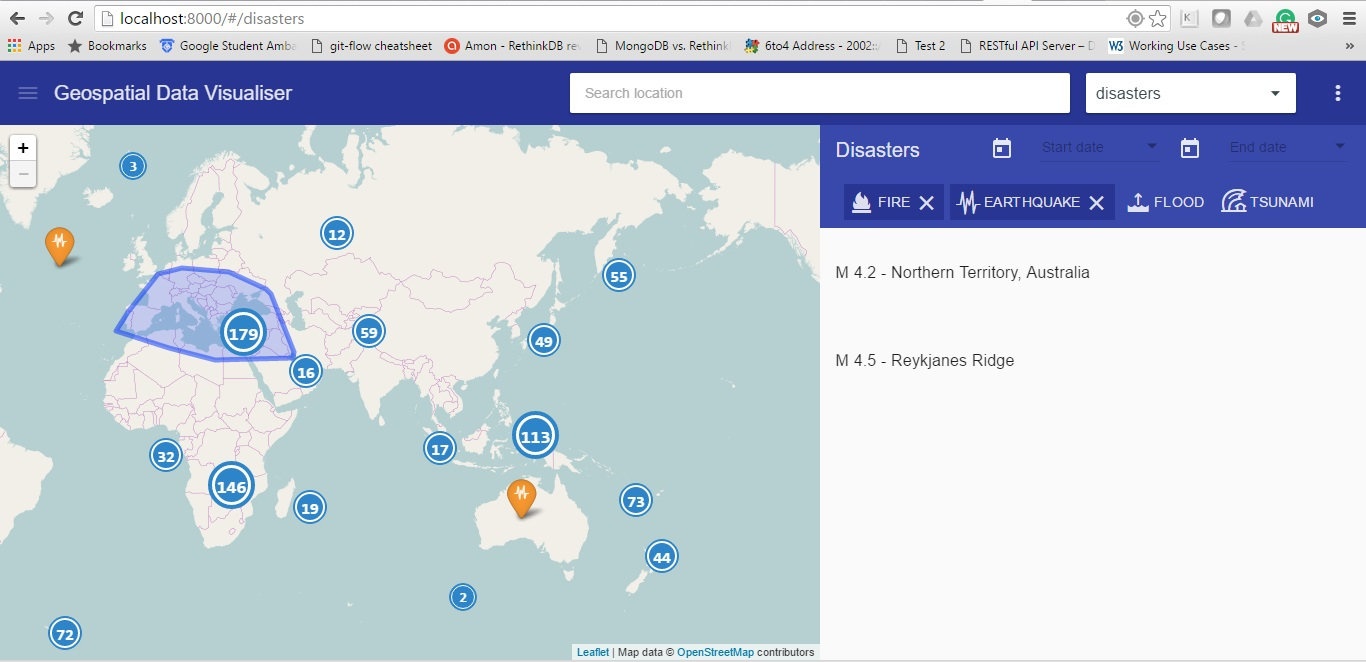
\includegraphics[width=\textwidth]{disaster4} \\[0.5cm]
		When you click one of these blue icons, the system perform a zoom service to the location of that icon. This then reveals more blue icons or disasters hidden by the clustering feature. By clicking another blue icon another zoom service is performed again etc.
	\end{enumerate}
\subsubsection{Weather Center}
\subsubsection{Map Features}